\documentclass[0_main]{subfiles}

\begin{document}

\ifEn
    \section{Basic Concepts of Continuous Optimization}
\else
    \section{連続最適化の基本概念}
\fi
\label{sec:background_basic}

\ifEn
    One of the central goals of numerical optimization is to determine decision variables that optimize a given quantitative measure.
    Examples of such measures include control stability, operational efficiency, and prediction error, each quantifying the quality of various phenomena or systems.
    These measures are typically modeled by an objective function that maps decision variables to real numbers.
\else
    数理最適化の中心的な意義の一つは、与えられた定量的な指標を最適化する決定変数を求めることである。
    そのような指標の例としては制御の安定性、運用の効率性、予測誤差など、さまざまな現象やシステムの品質を定量化したものが挙げられる。
    これらの指標は通常、決定変数を実数に写像する目的関数としてモデル化される。
\fi

\ifEn
    In this chapter, we define $f \colon \mathbb{R}^n \to \mathbb{R}$ as an objective function of class $C^2$, where $n$ denotes the dimension of the decision variables. We consider the following unconstrained optimization problem:
\else
    本章では、目的関数を $C^2$ 級の関数 $f \colon \mathbb{R}^n \to \mathbb{R}$ とし、また $n$ を決定変数の次元と定める。 この時、次の無制約最適化問題を考える:
\fi
\begin{equation*}
    \underset{x \in \mathbb{R}^n}{\text{minimize}} \quad f(x).
\end{equation*}
\ifEn
    In this section, we provide fundamental definitions and properties related to this optimization problem.
\else
    本節では、この最適化問題に関する基本的な定義と性質をまとめる。
\fi

\ifEn
    \subsection{Convexity and Strong Convexity}
\else
    \subsection{凸性と強凸性}
\fi

\ifEn
    The notions of convexity and strong convexity are fundamental in optimization theory.
    Assume that $f$ is of class $C^2$.
    The function $f$ is convex and strongly convex if and only if the following definitions hold for any two points $x,y \in \mathbb{R}^n$:
\else
    凸性(convexity)と強凸性(strong convexity)は最適化理論の基本概念である。
    $f$ は $C^2$ 級と仮定する。
    関数 $f$ が凸あるいは強凸であることは、任意の $x,y \in \mathbb{R}^n$ について次の定義が成り立つこととそれぞれ同値である:
\fi
\begin{align*}
    \text{(convex)} \quad
    f(y) & \ge f(x)+\nabla f(x)^\top (y-x),                           \\
    \text{($\mu$-strongly convex)} \quad
    f(y) & \ge f(x)+\nabla f(x)^\top (y-x)+\frac{\mu}{2}\norm{y-x}^2,
\end{align*}
\ifEn
    where $\mu>0$ is a constant.
    Strong convexity indicates that, in addition to convexity, the objective function has uniformly positive curvature.
    Examples of convex and strongly convex functions are shown in \cref{fig:convexity_comparison}.
\else
    ただし、 $\mu>0$ は定数である。
    強凸性は、凸性に加えて目的関数が一様に正の曲率を持つことを意味する。
    凸関数と強凸関数の例を \cref{fig:convexity_comparison} に示した。
\fi

\begin{figure}[t]
    \centering
    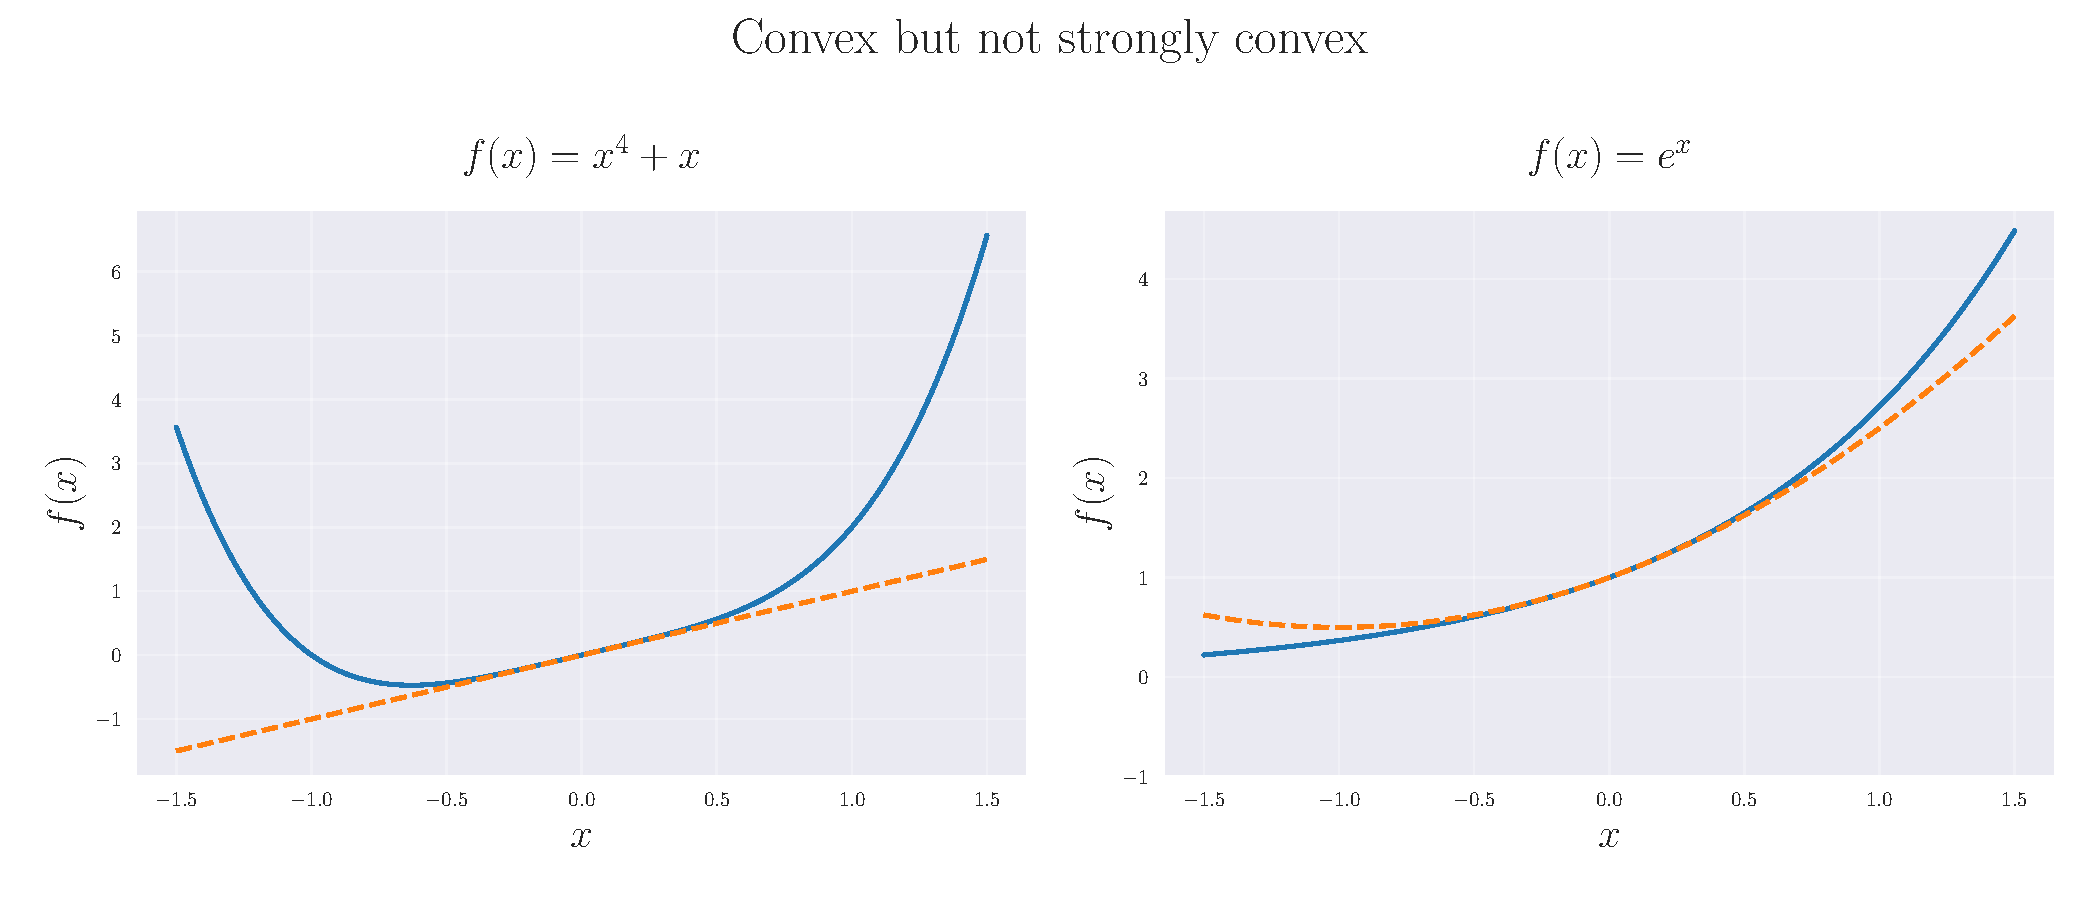
\includegraphics[width=\textwidth]{../imgs/quasi_newton/convexity_comparison_convex.pdf}
    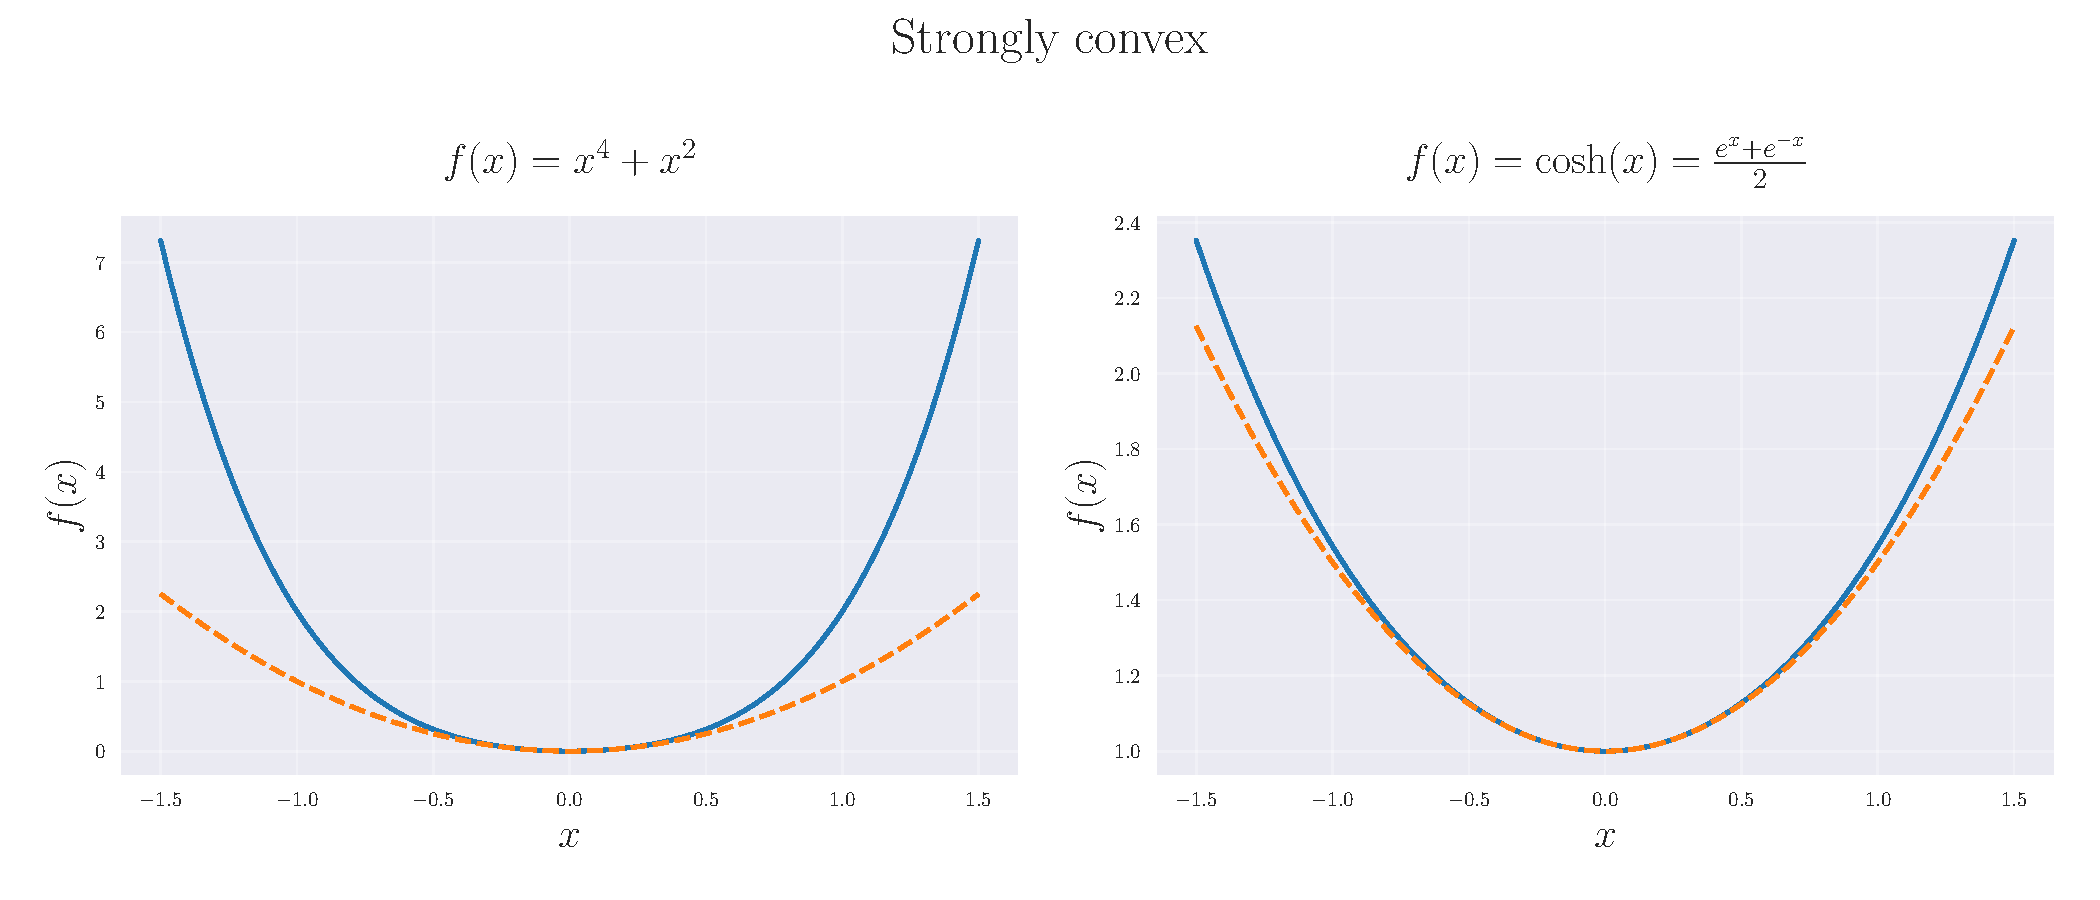
\includegraphics[width=\textwidth]{../imgs/quasi_newton/convexity_comparison_strongly_convex.pdf}
    \caption{
        \ifEn
            Examples of convex and strongly convex functions.
            The dashed line shows the quadratic approximation at $x=0$.
            The upper two functions are convex but not strongly convex.
            The lower two functions are strongly convex, and there exists $\mu>0$ that satisfies the definition of the strong convexity.
        \else
            凸関数と強凸関数の例。
            破線は $x=0$ における二次近似を示す。
            上の2つの関数は凸であるが強凸ではない。
            下の2つの関数は強凸であり、強凸性の定義を満たす $\mu>0$ が存在する。
        \fi
    }
    \label{fig:convexity_comparison}
\end{figure}

\subsection{Positive Definiteness of the Hessian}

\ifEn
    Next, we show how convexity and strong convexity relate to the definiteness of the Hessian matrix $\nabla^2 f(x)$.
    Let $A$ be a symmetric matrix in $\mathbb{R}^{n \times n}$. A matrix $A$ is called positive or negative definite (or semi-definite) based on the following conditions:
\else
    次に、凸性および強凸性がヘッセ行列 $\nabla^2 f(x)$ の正定値性とどのように関係するかを示す。
    $A$ を $\mathbb{R}^{n \times n}$ の対称行列とする。行列 $A$ が正定値(positive definite)・負定値(negative definite) (または半正定値(positive semi-definite)・半負定値(negative semi-definite))であるとは、次の条件で定義される:
\fi
\begin{align*}
    \text{(positive definite)} \quad      & v^\top A v > 0 \quad \forall v \in \mathbb{R}^n \setminus \{ 0 \}, \\
    \text{(positive semi-definite)} \quad & v^\top A v \ge 0 \quad \forall v \in \mathbb{R}^n,                 \\
    \text{(negative definite)} \quad      & v^\top A v < 0 \quad \forall v \in \mathbb{R}^n \setminus \{ 0 \}, \\
    \text{(negative semi-definite)} \quad & v^\top A v \le 0 \quad \forall v \in \mathbb{R}^n.
\end{align*}
\ifEn
    A matrix is indefinite if it is neither positive nor negative definite.
    For matrices $A,B \in \mathbb{R}^{n \times n}$, the notation $A \succeq B$ indicates that $A-B$ is positive semi-definite.
    In particular, if $B$ is a zero matrix, we simply write $A \succeq 0$.
    We similarly define $\preceq$ for negative semi-definiteness.
    For $\mu \geq 0$, the condition $A \succeq \mu I$ is equivalent to $v^\top A v \ge \mu \norm{v}^2$ for all $v \in \mathbb{R}^n$.
    It directly implies that all eigenvalues of $A$ are at least $\mu$, which in turn implies that the operator norm $\norm{A}$ is at least $\mu$, i.e., $\norm{A} \geq \mu$.
\else
    正定値でも負定値でもない行列は不定値(indefinite)と呼ぶ。
    行列 $A,B \in \mathbb{R}^{n \times n}$ に対して、$A \succeq B$ は $A-B$ が半正定値であることを表す。
    特に $B$ が零行列のときは $A \succeq 0$ と書く。
    同様に、$\preceq$ は半負定値に対して定義する。
    $\mu \geq 0$ に対し、$A \succeq \mu I$ はすべての $v \in \mathbb{R}^n$ について $v^\top A v \ge \mu \norm{v}^2$ と同値である。
    これは $A$ のすべての固有値が少なくとも $\mu$ であることを意味し、さらに作用素ノルムについて $\norm{A} \geq \mu$ であることを導く。
\fi

\ifEn
    We can relate convexity and strong convexity to the definiteness of the Hessian as follows.
\else
    凸性および強凸性とヘッセ行列の正定値性との関係は次のとおりである。
\fi
\begin{proposition}\label{prop:convexity-hessian}
    \ifEn
        Let $f \colon \mathbb{R}^n \to \mathbb{R}$ be of class $C^2$. Then
        \begin{itemize}
            \item $f$ is convex if and only if $\nabla^2 f(x)\succeq0$ holds for all $x \in \mathbb{R}^n$.
            \item $f$ is $\mu$-strongly convex if and only if $\nabla^2 f(x)\succeq\mu I$ holds for all $x \in \mathbb{R}^n$.
        \end{itemize}
    \else
        $f \colon \mathbb{R}^n \to \mathbb{R}$ を $C^2$ 級とする。このとき
        \begin{itemize}
            \item $f$ が凸であることと、任意の $x \in \mathbb{R}^n$ で $\nabla^2 f(x)\succeq0$ が成り立つことは同値である。
            \item $f$ が $\mu$-強凸であることと、任意の $x \in \mathbb{R}^n$ で $\nabla^2 f(x)\succeq\mu I$ が成り立つことは同値である。
        \end{itemize}
    \fi
\end{proposition}
\begin{proof}
    \ifEn
        First, let $\mu>0$ and assume $\nabla^2 f(x)\succeq \mu I$ for all $x \in \mathbb{R}^n$.
        By the fundamental theorem of calculus, for any $x,y \in \mathbb{R}^n$, we have
    \else
        まず $\mu>0$ とし、任意の $x \in \mathbb{R}^n$ に対して $\nabla^2 f(x)\succeq \mu I$ が成り立つと仮定する。
        微分積分学の基本定理より、任意の $x,y \in \mathbb{R}^n$ について次が成り立つ:
    \fi
    \begin{equation*}
        f(y)
        = f(x)+\nabla f(x)^\top (y-x)
        +\frac{1}{2} \int_0^1 (y-x)^\top \nabla^2 f(x+t(y-x))(y-x) \mathrm{d}t.
    \end{equation*}
    \ifEn
        By the assumption $\nabla^2 f(x)\succeq \mu I$, we have
    \else
        また、仮定 $\nabla^2 f(x)\succeq \mu I$ から次が得られる:
    \fi
    \begin{equation*}
        \int_0^1 (y-x)^\top \nabla^2 f(x+t(y-x))(y-x) \mathrm{d}t
        \ge \int_0^1 \mu\norm{y-x}^2 \mathrm{d}t
        = \mu\norm{y-x}^2.
    \end{equation*}
    \ifEn
        Thus, combining these results gives the definition of $\mu$-strong convexity.
    \else
        以上の結果を合わせると、$\mu$-強凸性の定義が導かれる。
    \fi

    \ifEn
        Conversely, assume that $f$ is $\mu$-strongly convex.
        For any $x \in \mathbb{R}^n, \, v \in \mathbb{R}^n$ and $t > 0$, letting $y=x \pm tv$ gives
    \else
        逆に、$f$ が $\mu$-強凸であると仮定する。
        任意の $x \in \mathbb{R}^n, \, v \in \mathbb{R}^n$ および $t>0$ に対し、$y=x \pm tv$ とおくと次を得る:
    \fi
    \begin{equation*}
        \begin{dcases}
            f(x + tv)\ge f(x) + t\nabla f(x)^\top v+\frac{\mu}{2}t^2\norm{v}^2, \\
            f(x - tv)\ge f(x) - t\nabla f(x)^\top v+\frac{\mu}{2}t^2\norm{v}^2.
        \end{dcases}
    \end{equation*}
    \ifEn
        By Taylor's theorem, there exists $s_\pm \in (0,1)$ such that
    \else
        テイラーの定理より、ある $s_\pm \in (0,1)$ が存在して次が成り立つ:
    \fi
    \begin{equation*}
        \begin{dcases}
            f(x + tv) = f(x) + t\nabla f(x)^\top v + \frac{1}{2} t^2 v^\top \nabla^2 f(x + s_+ t v) v, \\
            f(x - tv) = f(x) - t\nabla f(x)^\top v + \frac{1}{2} t^2 v^\top \nabla^2 f(x - s_- t v) v.
        \end{dcases}
    \end{equation*}
    \ifEn
        Combining these results gives
    \else
        これらの結果を合わせると次を得る:
    \fi
    \begin{equation*}
        v^\top \frac{\nabla^2 f(x+ s_+ t v) + \nabla^2 f(x - s_- t v)}{2} v \ge \mu \norm{v}^2.
    \end{equation*}
    \ifEn
        Letting $t \to 0$ and using the continuity of $\nabla^2 f$ from the $C^2$ assumption gives
    \else
        $t \to 0$ とし、$f$ が $C^2$ 級という仮定による $\nabla^2 f$ の連続性を用いると次を得る:
    \fi
    \begin{equation*}
        v^\top \nabla^2 f(x) v \ge \mu \norm{v}^2.
    \end{equation*}
    \ifEn
        Because $v \in \mathbb{R}^n$ is arbitrary, we obtain $\nabla^2 f(x)\succeq \mu I$.
    \else
        $v \in \mathbb{R}^n$ は任意なので、$\nabla^2 f(x)\succeq \mu I$ を得る。
    \fi

    \ifEn
        Setting $\mu=0$ in the above shows the convex case in the same way.
    \else
        上記の議論で $\mu=0$ とすれば、同様に凸の場合も示される。
    \fi
    \myQED
\end{proof}

\ifEn
    Quadratic functions whose Hessians are positive definite, indefinite, and negative definite are illustrated in \cref{fig:pd}. One can visually confirm the correspondence between positive definiteness and convexity.
\else
    ヘッセ行列が正定値・不定値・負定値である二次関数を \cref{fig:pd} に示す。正定値性と凸性の対応関係を視覚的に確認できる。
\fi

\begin{figure}[t]
    \centering
    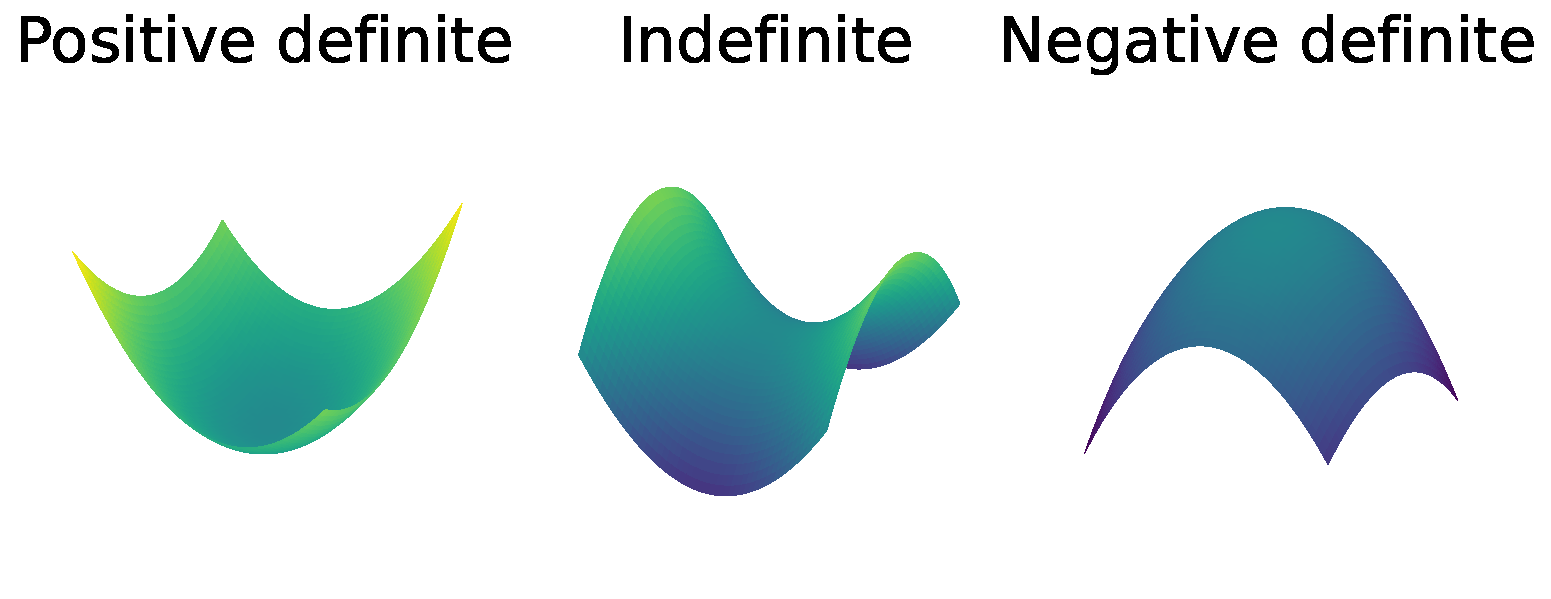
\includegraphics[width=\textwidth]{../imgs/quasi_newton/pd.pdf}
    \caption{
        \ifEn
            Quadratic model
            $f(x)=\frac{1}{2}(x - x_k)^\top H (x - x_k) + \nabla f(x_k)^\top (x - x_k) + f(x_k)$ in 2-dimensional space with Hessians $H$ which is (left) positive definite, (center) indefinite, (right) negative definite.
        \else
            二次モデル
            $f(x)=\frac{1}{2}(x - x_k)^\top H (x - x_k) + \nabla f(x_k)^\top (x - x_k) + f(x_k)$ を2次元空間で示したもの。
            ヘッセ行列 $H$ が (左)正定値、(中央)不定値、(右)負定値の場合を示す。
        \fi
    }
    \label{fig:pd}
\end{figure}

\ifEn
    \subsection{$L$-smoothness}
\else
    \subsection{$L$-平滑性}
\fi

\ifEn
    Finally, we introduce $L$-smoothness of functions.
    A function $f$ is $L$-smooth if and only if there exists a constant $L>0$ such that
\else
    最後に、関数の $L$-平滑性 ($L$-smoothness)を導入する。
    関数 $f$ が $L$-平滑であるとは、ある定数 $L>0$ が存在して
\fi
\begin{equation*}
    \norm{\nabla f(x)-\nabla f(y)} \le L\norm{x-y}
\end{equation*}
\ifEn
    holds for all $x,y$.
\else
    が任意の $x,y$ について成り立つことと同値である。
\fi

\ifEn
    The next proposition shows that $L$-smoothness can be characterized by the upper bound of the Hessian.
\else
    次の命題は、$L$-平滑性がヘッセ行列の上界で特徴づけられることを示す。
\fi
\begin{proposition}\label{prop:smoothness-hessian}
    \ifEn
        Let $f \colon \mathbb{R}^n \to \mathbb{R}$ be of class $C^2$. Then $f$ is $L$-smooth if and only if $\nabla^2 f(x)\preceq L I$ holds for all $x \in \mathbb{R}^n$.
    \else
        $f \colon \mathbb{R}^n \to \mathbb{R}$ を $C^2$ 級とする。このとき $f$ が $L$-平滑であることと、任意の $x \in \mathbb{R}^n$ で $\nabla^2 f(x)\preceq L I$ が成り立つことは同値である。
    \fi
\end{proposition}
\begin{proof}
    \ifEn
        Since $f$ is of class $C^2$, by the fundamental theorem of calculus, for any $x,y \in \mathbb{R}^n$, we have
    \else
        $f$ は $C^2$ 級なので、微分積分学の基本定理より任意の $x,y \in \mathbb{R}^n$ について次が成り立つ:
    \fi
    \begin{equation*}
        \nabla f(y) - \nabla f(x)
        = \int_0^1 \nabla^2 f(x+t(y-x))(y-x) \mathrm{d}t.
    \end{equation*}
    \ifEn
        Assume $\nabla^2 f(x)\preceq L I$ for all $x \in \mathbb{R}^n$.
        It implies that the operator norm of $\nabla^2 f(x)$ satisfies $\norm{\nabla^2 f(x)} \le L$, and thus
    \else
        任意の $x \in \mathbb{R}^n$ で $\nabla^2 f(x)\preceq L I$ と仮定する。
        このとき $\norm{\nabla^2 f(x)} \le L$ が成り立つので、
    \fi
    \begin{align*}
        \norm{\nabla f(y) - \nabla f(x)}
         & = \norm{\int_0^1 \nabla^2 f(x+t(y-x))(y-x) \mathrm{d}t}   &  & (\text{previous equation})   \\
         & \le \int_0^1 \norm{\nabla^2 f(x+t(y-x))(y-x)} \mathrm{d}t &  & (\text{triangle inequality}) \\
         & \le \int_0^1 L\norm{y-x} \mathrm{d}t                      &  & (\text{by assumption})       \\
         & = L\norm{y-x},
    \end{align*}
    \ifEn
        which proves the $L$-smoothness of $f$.
        Conversely, if $f$ is $L$-smooth, then for any $x \in \mathbb{R}^n$ and $v \in \mathbb{R}^n$, we have
    \else
        つまり、 $f$ の $L$-平滑性が示された。
        逆に、$f$ が $L$-平滑であるとすると、任意の $x \in \mathbb{R}^n$ と $v \in \mathbb{R}^n$ に対して次が成り立つ:
    \fi
    \begin{equation*}
        \norm{\nabla f(x+tv)-\nabla f(x)} \le L\norm{tv} = Lt\norm{v}.
    \end{equation*}
    \ifEn
        By Taylor's theorem, we also have
    \else
        さらにテイラーの定理より次が成り立つ:
    \fi
    \begin{equation*}
        \nabla f(x+tv)-\nabla f(x) = t \nabla^2 f(x) v + r(t),
    \end{equation*}
    \ifEn
        where $r(t)$ satisfies $\norm{r(t)}/t \to 0$ as $t \to 0$, and we can rewrite it as
    \else
        ただし、$r(t)$ は $t \to 0$ のとき $\norm{r(t)}/t \to 0$ を満たす。そして、これは次のように書き換えられる:
    \fi
    \begin{equation*}
        \nabla^2 f(x) v = \lim_{t \to 0} \frac{\nabla f(x+tv)-\nabla f(x) -r(t)}{t} = \lim_{t \to 0} \frac{\nabla f(x+tv)-\nabla f(x)}{t}.
    \end{equation*}
    \ifEn
        Taking the inner product  with $v$ gives
    \else
        $v$ との内積を取ると次が得られる:
    \fi
    \begin{align*}
        v^\top \nabla^2 f(x) v & = \lim_{t \to 0} \qty(\frac{\nabla f(x+tv)-\nabla f(x)}{t})^\top v                                                  \\
                               & \leq \lim_{t \to 0} \frac{\norm{\nabla f(x+tv)-\nabla f(x)}}{t} \norm{v} &  & (\text{Cauchy--Schwarz inequality})   \\
                               & \leq \lim_{t \to 0} \frac{L\norm{tv}}{t} \norm{v}                        &  & (\text{by $L$-smoothness definition}) \\
                               & = L \norm{v}^2.
    \end{align*}
    \ifEn
        Because $v \in \mathbb{R}^n$ is arbitrary, we obtain $\nabla^2 f(x)\preceq L I$.
    \else
        $v \in \mathbb{R}^n$ は任意なので、$\nabla^2 f(x)\preceq L I$ を得る。
    \fi
    \myQED
\end{proof}

\subsubsection{Baillon--Haddad Theorem}

\ifEn
{One of the useful properties of $L$-smooth functions is given by the following Baillon--Haddad theorem.
    Note that only $C^1$ differentiability is required here.}
\else
{$L$-smooth 関数の有用な性質の一つが次の Baillon--Haddad 定理である。
    ここでは $C^1$ の微分可能性だけを仮定する点に注意する。}
\fi
\begin{proposition}[Baillon--Haddad theorem]\label{prop:baillon_haddad}
    \ifEn
    {Let $f \colon \mathbb{R}^n \to \mathbb{R}$ be of class $C^1$. If $f$ is $L$-smooth and convex, then for all $x,y \in \mathbb{R}^n$, $\nabla f$ is $1/L$-cocoercive, i.e.,
        \begin{equation*}
            (\nabla f(x)-\nabla f(y))^\top (x-y) \ge \frac{1}{L} \norm{\nabla f(x)-\nabla f(y)}^2
        \end{equation*}
        for all $x,y \in \mathbb{R}^n$.}
    \else
    {$f \colon \mathbb{R}^n \to \mathbb{R}$ を $C^1$ 級とする。$f$ が $L$-smooth かつ凸であれば、任意の $x,y \in \mathbb{R}^n$ に対して $\nabla f$ は $1/L$-cocoercive であり、すなわち
        \begin{equation*}
            (\nabla f(x)-\nabla f(y))^\top (x-y) \ge \frac{1}{L} \norm{\nabla f(x)-\nabla f(y)}^2
        \end{equation*}
        が任意の $x,y \in \mathbb{R}^n$ について成り立つ。}
    \fi
\end{proposition}
\ifEn
{We refer to other literature for the proof \citep{bauschkeBaillonHaddadTheoremRevisited2009} \citep[Proposition 12.60]{rockafellarVariationalAnalysis1998}.}
\else
{証明は他の文献に譲る \citep{bauschkeBaillonHaddadTheoremRevisited2009} \citep[Proposition 12.60]{rockafellarVariationalAnalysis1998}。}
\fi
\ifEn
    One consequence of this theorem is that, for the sequences $\{ x_k \}$ generated by an optimization algorithm, defining
\else
    この定理の帰結として、最適化アルゴリズムが生成する列 $\{ x_k \}$ に対し、次を定義すると:
\fi
\begin{equation*}
    s_k \coloneqq x_{k+1}-x_k, \quad y_k \coloneqq \nabla f(x_{k+1}) - \nabla f(x_k)
\end{equation*}
\ifEn
    and applying Baillon--Haddad theorem with $x=x_{k+1}$ and $y=x_k$ yields
\else
    Baillon--Haddad 定理を $x=x_{k+1}$、$y=x_k$ に適用して次を得る:
\fi
\begin{equation*}
    s_k^\top y_k \ge \frac{1}{L} \norm{y_k}^2.
\end{equation*}
\ifEn
    This inequality is sometimes used in the analysis of update formulas in methods such as BFGS and L-BFGS.
\else
    この不等式は BFGS や L-BFGS などの更新公式の解析で用いられることがある。
\fi

\ifEn
    \subsubsection{Bound on Hessian Eigenvalues}
\else
    \subsubsection{ヘッセ行列の固有値のバウンド}
\fi

\ifEn
    The $L$-smoothness combined with $\mu$-strong convexity also provides bounds on the eigenvalues of the Hessian.
\else
    $L$-smoothness と $\mu$-強凸性を組み合わせると、ヘッセ行列の固有値に対するバウンドも得られる。
\fi
\begin{proposition}\label{prop:hessian-eigenvalue-bound}
    \ifEn
        Let $f \colon \mathbb{R}^n \to \mathbb{R}$ be of class $C^2$.
        If $f$ is $L$-smooth and $\mu$-strongly convex, then the eigenvalues of the Hessian $\nabla^2 f(x)$ are contained in the interval $[\mu, L]$ for all $x \in \mathbb{R}^n$.
    \else
        $f \colon \mathbb{R}^n \to \mathbb{R}$ を $C^2$ 級とする。
        $f$ が $L$-smooth かつ $\mu$-強凸であれば、任意の $x \in \mathbb{R}^n$ に対してヘッセ行列 $\nabla^2 f(x)$ の固有値は区間 $[\mu, L]$ に含まれる。
    \fi
\end{proposition}
\begin{proof}
    \ifEn
        By \cref{prop:convexity-hessian,prop:smoothness-hessian}, we have
    \else
        \cref{prop:convexity-hessian,prop:smoothness-hessian} より次が成り立つ:
    \fi
    \begin{equation*}
        \mu I \preceq \nabla^2 f(x) \preceq L I.
    \end{equation*}
    \ifEn
        This directly implies that the eigenvalues of $\nabla^2 f(x)$ are contained in the interval $[\mu, L]$.
    \else
        これより $\nabla^2 f(x)$ の固有値が区間 $[\mu, L]$ に含まれることが直ちに従う。
    \fi
    \myQED
\end{proof}
\ifEn
    As shown in \cref{prop:hessian-eigenvalue-bound},  the $L$-smoothness and $\mu$-strong convexity impose upper and lower bounds on the eigenvalues of the Hessian, respectively.
\else
    \cref{prop:hessian-eigenvalue-bound} で示したように、$L$-smoothness と $\mu$-強凸性はそれぞれヘッセ行列の固有値に上界と下界を与える。
\fi

\ifSubfilesClassLoaded{
    \bibliographystyle{plainnat}
    \bibliography{../L-BFGS.bib}
}{}

\end{document}
